\documentclass[11pt]{article}
\usepackage{geometry}                
\geometry{letterpaper}                   

\usepackage{graphicx}
\usepackage{amssymb}
\usepackage{epstopdf}
\usepackage{natbib}
\usepackage{amssymb, amsmath}
\usepackage{wrapfig}





%\title{Title}
%\author{Name 1, Name 2}
%\date{date} 

\begin{document}



\thispagestyle{empty}

\begin{center}

\includegraphics[width=5cm]{ETHlogo.eps}

\bigskip


\bigskip


\bigskip


\LARGE{ 	Lecture with Computer Exercises:\\ }
\LARGE{ Modelling and Simulating Social Systems with MATLAB\\}

\bigskip

\bigskip

\small{Project Report}\\

\bigskip

\bigskip

\bigskip

\bigskip


\begin{tabular}{|c|}
\hline
\\
\textbf{\LARGE{Cholera Epidemic in Haiti 2010}}\\
\\
\hline
\end{tabular}
\bigskip

\bigskip

\bigskip

\LARGE{Nicolas Stocker 

Benedict Borer

Benjamin Pluess 

Lukas Buehler}



\bigskip

\bigskip

\bigskip

\bigskip

\bigskip

\bigskip

\bigskip

\bigskip

Zurich\\
\today\\
\end{center}



\newpage

%%%%%%%%%%%%%%%%%%%%%%%%%%%%%%%%%%%%%%%%%%%%%%%%%

\newpage
\section*{Agreement for free-download}
\bigskip


\bigskip


\large We hereby agree to make our source code for this project freely available for download from the web pages of the SOMS chair. Furthermore, we assure that all source code is written by ourselves and is not violating any copyright restrictions.

\begin{center}

\bigskip


\bigskip


\begin{tabular}{@{}p{3.3cm}@{}p{6cm}@{}@{}p{6cm}@{}}
\begin{minipage}{3cm}

\end{minipage}
&
\begin{minipage}{6cm}
\vspace{2mm} \large Nicolas Stocker 


 \vspace{\baselineskip}

\end{minipage}
&
\begin{minipage}{6cm}

\large Benjamin Pluess

\end{minipage}
\end{tabular}

\bigskip
\bigskip
\bigskip

\begin{tabular}{@{}p{3.3cm}@{}p{6cm}@{}@{}p{6cm}@{}}
\begin{minipage}{3cm}

\end{minipage}
&
\begin{minipage}{6cm}
\vspace{2mm} \large Benedict Borer 


 \vspace{\baselineskip}

\end{minipage}
&
\begin{minipage}{6cm}

\large Lukas Buehler

\end{minipage}
\end{tabular}


\end{center}
\newpage

%%%%%%%%%%%%%%%%%%%%%%%%%%%%%%%%%%%%%%%



% IMPORTANT
% you MUST include the ETH declaration of originality here; it is available for download on the course website or at http://www.ethz.ch/faculty/exams/plagiarism/index_EN; it can be printed as pdf and should be filled out in handwriting


%%%%%%%%%% Table of content %%%%%%%%%%%%%%%%%

\tableofcontents

\newpage

%%%%%%%%%%%%%%%%%%%%%%%%%%%%%%%%%%%%%%%



\section{Abstract}

\section{Individual contributions}

\section{Introduction and Motivations}
\textit{The Shock}

\begin{wrapfigure}{r}{5cm}
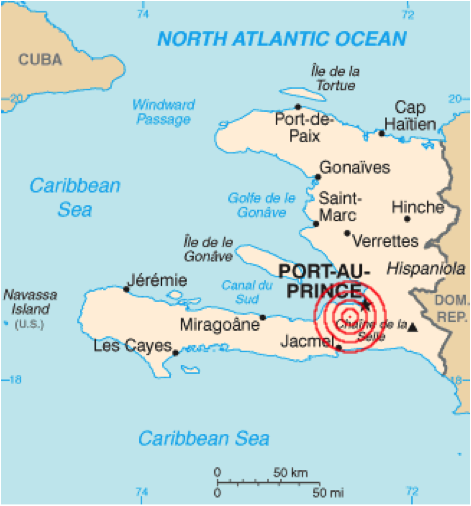
\includegraphics[scale=0.8]{Bilder/KarteHaiti.png}
\caption{Hier steht die Beschreibung des Bildes}%
\end{wrapfigure}
12. January 2010, 16.53 local time in Haiti: during one minute the earth is shaking with magnitude 7.0  (on the Moment magnitude scale) with an epicentre 25 Km west of Haiti’s capital Port-au-Prince. Followed by at least 52 aftershocks  this earthquake is the most dramatic in the 21. Century: the Haitian government estimated that 316’000 people had died , one million people lost their home  and 3.2 million are directly affected.
\\[1em]
\noindent \textit{Geological overview}

The quake was located on the active plate boundary with the Caribbean Tectonic Plate shifts eastwards relative to the North American Plate. This causes a highly dangerous strike-slip-fault system here with the southern active Enriquillo-Plantain-Garden-fault. The quake is caused by a rupture of this system, which has been blocked for the last 2500 years, loading stress
\\[1em]
\noindent\textit{Primary impacts}

As Haiti is one of the poorest country in the Western Hemisphere  the economy is highly vulnerable to natural disasters. In addition to earthquakes, the “island of Hispaniola” shared by the Dominican Republic and Haiti, has often been stroked by Hurricanes. 
\newline
The huge devastation and damage in the whole country, but especially in the region of the capital, destroy not only human life, furthermore infrastructure, which would have been necessary to respond to the disaster. Not only all hospitals in the capital, as well air, water and land transport facilities and the communication system was destroyed. As well a lot off the public and government buildings were damaged (e.g. the National Assembly, the Palace of Justice and the Supreme Court)
\\[1em]
\noindent\textit{The time afterwards}

In the following months after the earthquake many people slept in the streets because their houses has been destroyed or they were feared that their buildings won’t survive upcoming aftershocks. Slow distribution of recourses resulted in violence and some people began with plundering.
\newline
The earthquake destroyed thousands of families and made collapse a whole social system and destroyed economic interactions in a country. Anarchy and a right-free area was the result. Haitians dramatic fight for survival began in the silent seconds after the earthquake and still goes on.
\\[1em]
\noindent\textit{Upcoming problem: Cholera}

During the period of reconstruction in October 2010 Haiti was confronted by a new dangerous problem: a cholera epidemic broke out! 
\newline
Cholera is a bacterial infection caused by a bacterium named as “Vibro cholerae”. The symptoms are mainly watery diarrhoea and vomiting. The transmission occurs generally by drinking infected water. Cholera doesn’t have to be lethal but requires an appropriate treatment in a hospital. In Haiti in January 2012 some 7025 deaths by Cholera have been reported 
The source of the illness still is not clearly identified, but localized in de Artibonite River about 100 Km north of Port-Au-Prince (The affected victims had drunk water from the infected river). Some UN investigators did researches, hoping to find the real source from the Epidemic and they are guessing the initial strain was imported by UN peacekeeper from Nepal . The Nepali soldiers may be the source of the outbreak as wastewater from their outhouses at their base flowed into and contaminated the Artibonite River  . However who brought the origin strain to Haiti is not of primary importance, rather than to control the plague and this is still one of the most important priority nowadays in Haiti.
\\[1em]
\noindent\textit{Motivation}

By the end of October 2010 the Cholera epidemic accomplished four out of ten Haitian’s departments: Artibonite, Centre, Nord and Ouest. That includes as well the Capital , especially the slum district “Cité Soleil” . In the following days Cholera was spread all over the country and infected thousands of peoples. The tragedy of Haiti is not only a “simple” earthquake; it is more a battle rebuilding a country affected by complicating circumstances such as the Cholera Epidemic. 
\newline
Our aim is to understand the fast spreading of the dangerous illness Cholera and to implement a mathematical model, which is able to predict the expansion of such an epidemic in space and time. We believe to help getting a deeper understanding of the interaction of a human – environment interaction and so to do our part for protecting human lives in further catastrophic events.


\section{Description of the Model}

A general model for epidemics was established by Kermack and McKendrick over 80 years ago (1927). It is a representative of the so called SIR models. SIR stands for the three groups a population is divided into; susceptible, infected and removed persons for the particular disease. The model makes the assumptions that the population size is constant, no incubation period exists which means that individuals fall ill the moment they are infected and the time of infectivity is the same as the duration of the clinical disease (powerpoint presentation MSSSM). This implies that infected individuals are always infectious and the other way around. Infected and infectious have therefore to be seen as descriptions of the same state. Because in reality those expressions are not equivalent either one of them is used in a logical appropriate manner. Furthermore after having been infected once, individuals become completely immune to the disease in question (Kermack and McKendrick, 1927). Kermack and McKendrick and have used plague as an example of an epidemic which can be modeled by their work. Since then other epidemics have been modeled by similar frameworks that can be counted as part of the SIR models.
The Kermack-McKendrick model equations are the following:
\begin{equation*}
\dfrac{dS}{dt}=-\beta X(t)S(t)
\end{equation*}
\begin{equation*}
\dfrac{dX}{dt}=\beta X(t)S(t)-\gamma X(t]
\end{equation*}
\begin{equation*}
\dfrac{dR}{dt}=\gamma X(t)]
\end{equation*}
S, X and R are the numbers of susceptible, infectious and removed persons respectively. Removed means that those people have either died from the disease or they have recovered and as a result are perfectly immune now. Either way they are no longer candidates to become infected and they do not belong to the infectious anymore.
\linebreak 
Here $\beta$ stands for the infection rate and $\gamma$ for the immunity (or death) rate. It is the inverse value of the average duration of infectiousness. If $\beta$ and $\gamma$ are constants the spreading of an epidemic that is modelled with this concept can only decrease or be stopped when enough individuals have been moved from the susceptible to the removed compartment (becoming infectious and then being removed because of death or recovery); a decrease in the value of the susceptible compartment ($ S $) is going to lower the term $\beta X(t)S(t)$ which leads to a decrease of the value of infectious ($ X $) eventually stopping the epidemic.
\\For diseases that are transmitted through water and person-to-person contact an extension of the SIR model was developed by Tien and Earn (Verweis zu ihrem paper). The main difference is the introduction of a fourth compartment $ W $ which represents the waterbody. The water compartment can be contaminated by infectious people and susceptible individuals can be infected by the contaminated water compartment. This water compartment can improve the quality of predictions for diseases that are mainly transmitted through ingestion of contaminated water.
\linebreak
Another new feature of the model is the introduction of natural death terms in every compartment with humans (all compartments expect $ W $) and a corresponding birth term in the susceptible compartment. These terms are chosen so that the total number of individuals in all compartments with humans stays constant.
The model equations are the following:
\begin{equation*}
\dfrac{dS}{dt}=\mu N-b_{W}WS-b_{I}SX-\mu S 
\end{equation*}
\begin{equation*}
\dfrac{dX}{dt}=b_{W}WS+b_{I}SX-\gamma I-\mu X
\end{equation*}
\begin{equation*}
\dfrac{dR}{dt}=\gamma X-\mu R
\end{equation*}
\begin{equation*}
\dfrac{dW}{dt}=\alpha X-\xi W
\end{equation*}
$ \mu $ is the parameter for natural deaths and the birth rate. Natural deaths occur in every human compartment while all babies are born into the susceptible compartment.$ b_{W} $ represents the rate of infection by water-to-person contact whereas $ b_{I} $ is the rate of infection for person-to-person contact.$ \dfrac{1}{\gamma } $ is the mean infectious period.So $ \gamma $ stands for the rate of infectious persons to either die or recover and become immune. In both cases those individuals change from the $ X $ to the $ R $ compartment. $ \alpha $ is the pathogen shedding rate from infectious persons into the water compartment while $ \xi $ denotes the decay rate of the particular pathogen in water.
\\
\begin{center}
\begin{figure}
\centerline{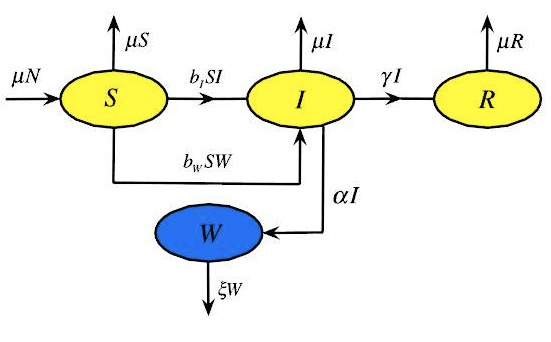
\includegraphics[scale=0.5]{Bilder/flow_diagramm_siwr_copia.png}}
\caption{Hier steht die Beschreibung des Bildes}
\end{figure}
\end{center}
The flow diagram gives an overview of the parameters and the roles they play in this model. (Taken from Tien and Earn).
The model equations that we used were rescaled as recommended by Tien and Earn. Rescaling has some advantages, one of which being the possibility to directly compare different epidemics with different populations. Another one is the absence of units in $ S, X, W, R $. Used for rescaling is the total population number $ N $. The new properties have the following relationship with the old ones: 
\begin{equation*}
s=\dfrac{S}{N} ,	  x=\dfrac{X}{N} ,	  r=\dfrac{R}{N} ,     w=\dfrac{W}{N}\dfrac{\xi}{\alpha} 
\end{equation*}
\begin{equation*}
\dfrac{ds}{dt}=\mu -\beta_{W}ws-\beta_{I}sx-\mu s
\end{equation*}
\begin{equation*}
\dfrac{dx}{dt}=\beta_{W}ws+\beta_{I}sx-\gamma x-\mu x
\end{equation*}
\begin{equation*}
\dfrac{dr}{dt}=\gamma x-\mu r
\end{equation*}
\begin{equation*}
\dfrac{dw}{dt}=\xi (x-w) 
\end{equation*}
Because $ W $ was replaced by the expression $ wN\dfrac{\alpha}{\xi} $ which is a bit more complicated than just $ wN $ parameters in expressions with a former capital $ W $ are replaced by new parameters. The differential equation for the water compartment has become simpler as only one parameter $ \xi $ is needed from now on. Two new parameters are introduced to replace $ b_{W} $ and $ b_{I} $ by $ \beta_{W}=b_{W}N\dfrac{\alpha}{\xi} $ and $ \beta_{I}=b_{I}N $ respectively.
"The basic reproductive number $ R_{0} $ is defined as the expected number of secondary infections that result from introducing a single infected individual into an otherwise susceptible population. $ R_{0} $ is a fundamental quantity in mathematical epidemiology, which-in the deterministic limit-dictates whether a newly invading pathogen will cause a disease outbreak" (direct quote Tien and Earn). For this model the equation $ R_{0}=\dfrac{\beta_{I}+\beta_{W}}{\gamma+\mu} $ holds.\\
This model can be applied to the case of a population  that is spatially separated into different parts. In our case these were the ten departments of Haiti. The only additional term which was added for this approach gives the person-to-person infections by infectious individuals of different departments. So the susceptible population of every department could be infected by the infectious population or contaminated water of their own department or infectious individuals of other departments. 
\newline The last term accounts for people that move or travel around. To consider the distances between different compartments a gravity-model was used. Parameter $ \theta $ depends on the population of the two departments in question and on the distance between their capital cities. The concept is essentially the same as for the gravity equation: $ \theta_{ij}=\kappa\dfrac{p_{i}p_{j}}{d^{n}} $. $ p_{i} $ and $ p_{j} $ are population sizes of different departments, $ d $ is given by the distance between the capital cities of the two departments in question, $ n $ influences how strong transmission depends on distance and $ \kappa $ determines how important the transmission between departments is thought to be. With this equation a between department transmission rate $ \theta_{ij} $ can be calculated for every possible constellation. With 10 departments this results in 90 different $ \theta_{ij} $ one for every possible combination. 
\newline Because of the shape of Haiti it was divided into a northern and a southern part when determining these distances. Ouest was thought to be the link between those two parts where all travellers had to pass through. So distances of departments that did not belong to the same part where taken as the sum of distances between the capital city of the department in the northern part and the capital city of Ouest and the distance between the capital cities of Ouest and the department in the southern part.\\
The equation for the model with different departments (indicated by the index $ i $ are the following:
\begin{center}
$ \dfrac{ds_{i}}{dt}=\mu -\beta_{W}w_{i}s_{i}-\beta_{I}s_{i}x_{i}-s_{i}\sum_{j=1}^{10}\theta_{ij}x_{j}-\mu s_{i} $
\linebreak
$ \dfrac{dx_{i}}{dt}=\beta_{W}w_{i}s_{i}-\beta_{I}s_{i}x_{i}+s_{i}\sum_{j=1}^{10}\theta_{ij}x_{j}
-\gamma x_{i}-\mu x_{i} $
\linebreak
$ \dfrac{dr_{i}}{dt}=\gamma x_{i}-\mu r_{i} $
\linebreak
$ \dfrac{dw_{i}}{dt}=\xi (x_{i}-w_{i}) $
\linebreak
\end{center}
Another parameter $ \lambda $ is introduced to summarise all the effects of the pathogen like person-to-person and water-to-person transmission within a compartment and person-to-person transmission between compartments. While this may give a better overview about the model it hides the non-linear terms. It is important to keep in mind that $ \lambda $ includes parameters as well as variables! 

\begin{center}
$ \lambda_{i}=\beta_{W}w_{i}+\beta_{I}x_{i}+\sum_{j=1}^{10}\theta_{ij}x_{j}
$
\end{center}
$ \lambda_{i} $ represents the total force of infection in the $ i $th department. The model equations with $ \lambda $ included look the following:
\begin{center}
$ \dfrac{ds_{i}}{dt}=\mu -\lambda_{i}s_{i}-\mu s_{i} $
\linebreak
$ \dfrac{dx_{i}}{dt}=\lambda_{i}s_{i}-\gamma x_{i}-\mu x_{i} $
\linebreak
$ \dfrac{dr_{i}}{dt}=\gamma x_{i}-\mu r_{i} $
\linebreak
$ \dfrac{dw_{i}}{dt}=\xi (x_{i}-w_{i}) $
\end{center}
\begin{figure}
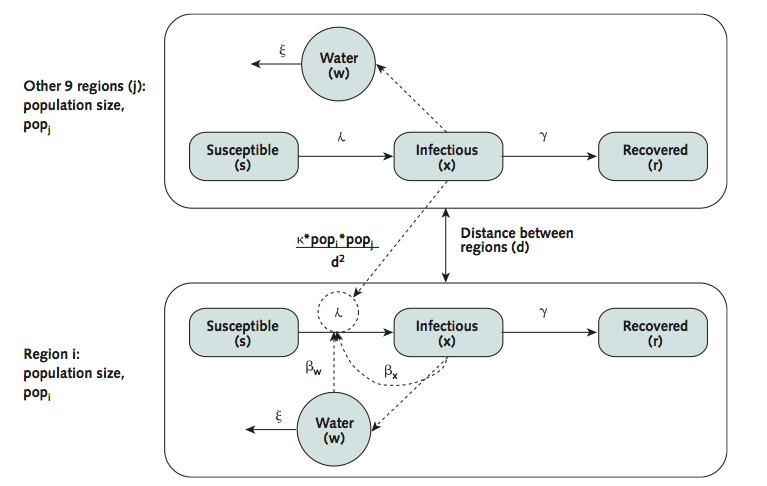
\includegraphics[scale=1]{Bilder/figure_model.png} \\
\caption{Summary of the used model}
\end{figure}
 The figure summarizes the processes and compartments and shows which parameter accounts for which process. Each of the 10 departments consists of the 4 compartments susceptible (s), infectious (x), removed (r) and water (w). Birth and natural deaths ($ \mu $) are left out in the figure. $ n $ in the gravity model is set to 2 here.
\linebreak
Right calibration of every model is crucial to produce results that are close to reality. As the SIWR model has several parameters this task is quite difficult. With the onset of disease-control interventions the basic reproductive number $ R_{0} $ is bound to decrease. It can be taken into account by making $ R_{0} $ time-dependent. This effective reproductive number $ R_{t} $ could look like this:
\begin{center}


$ R_{t}=\dfrac{R_{0}}{(1+f)^{t}} $
\end{center}
Here $ f $ is a discount factor.
(Tuite et al.)

\section{Implementation}

\section{Simulation Results and Discussion}

\section{Summary and Outlook}



\noindent\textit{Outlook}

In response to the cholera outbreak, the Haiti government and partner agencies initiated emergency public health response activities aimed at treating suspected cholera cases and preventing new ones. Response activities included mass media cholera campaigns through radio and hygiene promotion activities by community health workers, distribution of water purification tablets and soap, and limited distribution of oral rehydration solution (ORS) sachets. (Quelle: http://www.ncbi.nlm.nih.gov/pmc/articles/PMC3310585/?tool=pubmed)

Regarding to the mass media campaign, it seems helpful to know how the cholera bacteria would distribute in waterways. With our model it is not yet possible to make an exact forecast about the distribution in water ways. Based on that knowledge the protection of population would be directly improved and should be used when cholera is threatening human beings.

Our model needs more detail information, which nowadays are not available. Hence we recommend a research during an epidemic with the aim to collect data of the consumation and quality of the water. In our case it would be helpful to know the quantity, localisation and exact time of an output (?) from water out of a contamined (?) river.

We belive such a dataset would highly improve the possibility of modelling a system like a cholera epidemic like that one in Haiti 2010.

\section{References}






\end{document}  
